\documentclass{article}
\usepackage{amsfonts, amsmath, amssymb, amsthm} % Math notations imported
\usepackage{enumitem}
\usepackage{graphicx}
\usepackage{setspace}
\usepackage{indentfirst}
\usepackage[margin=1in]{geometry}
\graphicspath{{./images/}} % Path to images

% \begin{figure}[htb!]
%      \centering
%      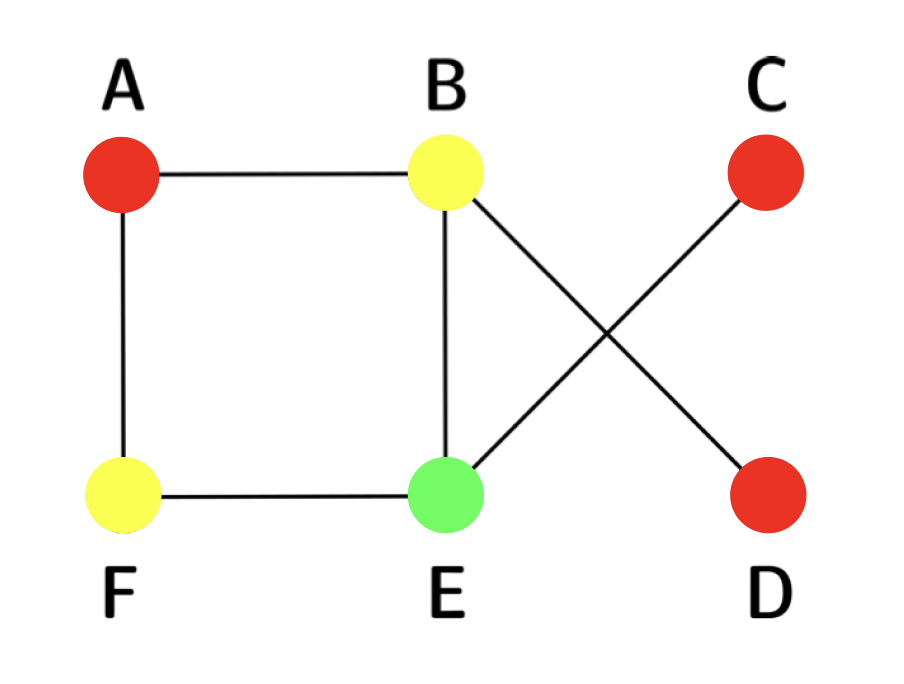
\includegraphics[scale=0.5]{coloring.png}
%      \caption{Coloring of the graph.}
% \end{figure}

% \begin{figure}[htb]
%     \qquad
%     \begin{minipage}{.4\textwidth}
%         \centering
%         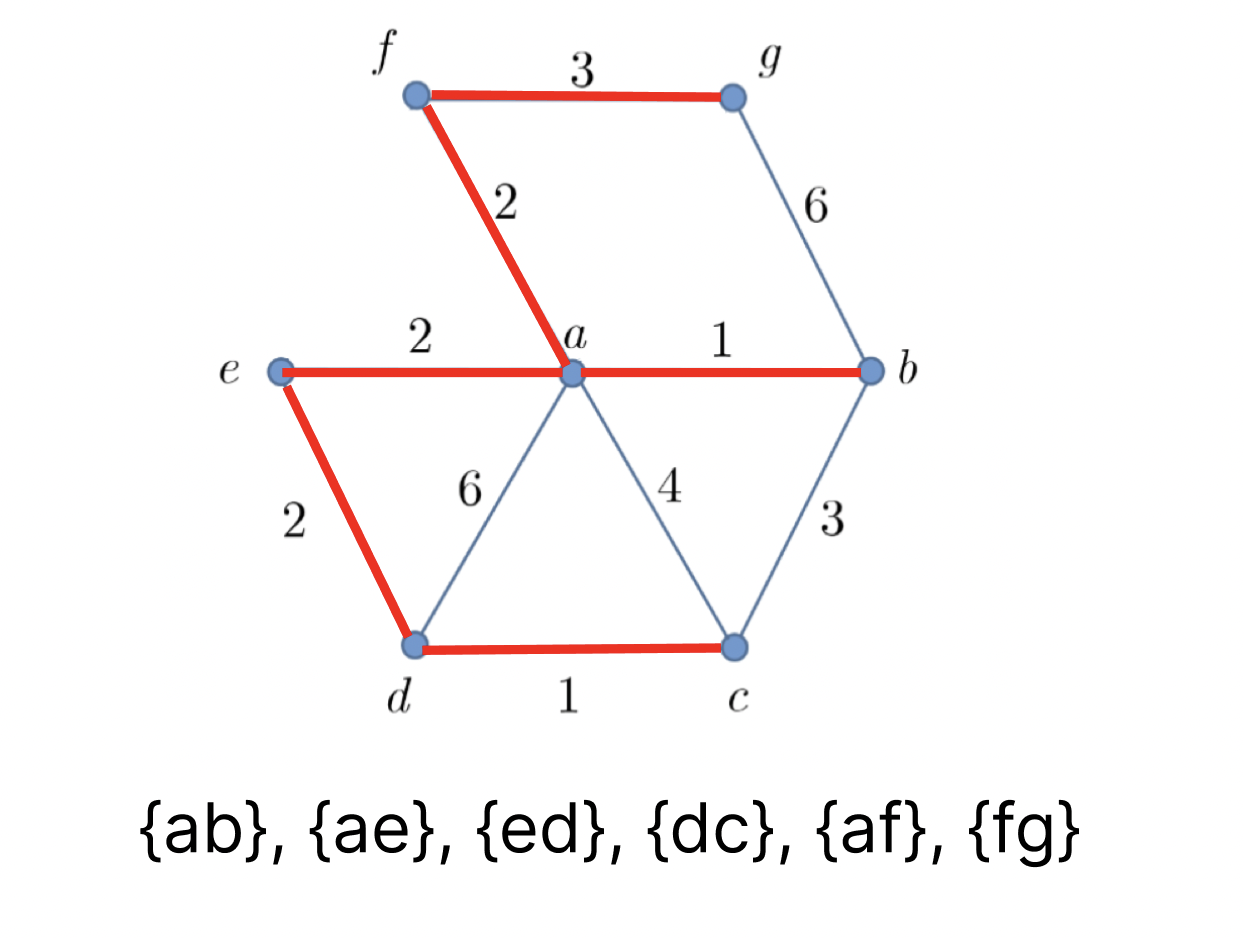
\includegraphics[scale=0.35]{prims.png}
%         \caption{}
%     \end{minipage}    
%     \qquad
%     \begin{minipage}{.4\textwidth}
%         \centering
%         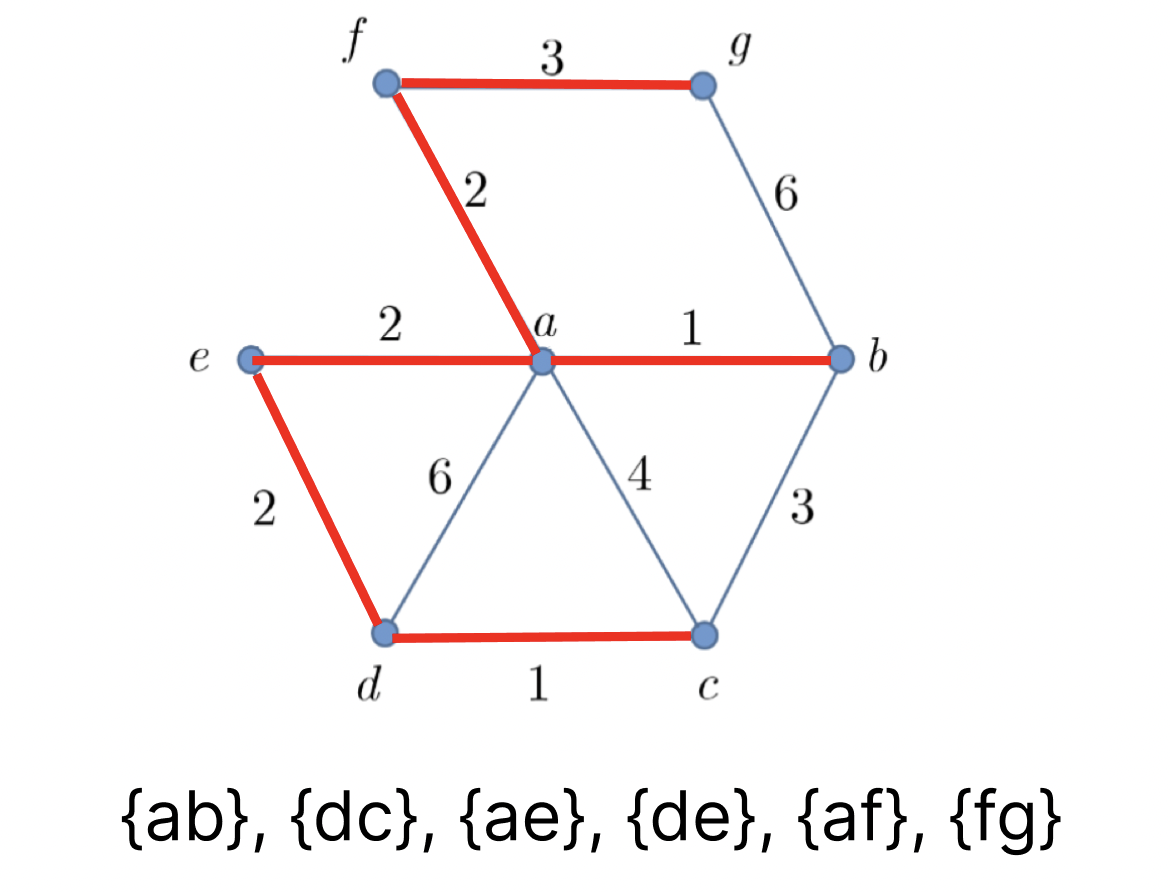
\includegraphics[scale=0.35]{kruskal.png}
%         \caption{}
%     \end{minipage}        
% \end{figure} 

\newtheorem{thm}{Theorem}
\newtheorem{proposition}[thm]{Proposition}
\newtheorem{cor}[thm]{Corollary}

% title information
\title{STAT 153 sketch}
\author{Neo Lee}
\date{}

\setstretch{1.15}
% main content
\begin{document} 

% placing title information; comment out if using fancyhdr
\maketitle 

Proof of null$(X)$ contains at least one non-zero vector $\eta$:

Since $p>n$, the column vectors are linear dependent. Denote $(v_1, \cdots, v_p)$ as the column 
vectors of $X$. Then, there are non trivial coefficients $(c_1, \cdots, c_p)$ such that
$$\sum_{i=1}^{p}c_iv_i=0.$$
Hence, $\eta = (c_1,\cdots, c_p)$ is a non-zero vector in null$(X)$.

Proof of $\hat{\beta}=\tilde{\beta}+\eta$ is also a least squares solution for $\eta\in 
\mathrm{null}(X)$:

Denote the prediction from $\tilde{\beta}$ as $\tilde{y} = X\tilde{\beta}$ with MSE = $y-\tilde{y}$. 
Then the prediction from $\hat{\beta}$
\begin{align}
    \hat{y} & = X\hat{\beta} \\
    & = X(\tilde{\beta}+\eta) \\
    & = X\tilde{\beta}+X\eta \\
    & = \tilde{y}+X\eta \\
    & = \tilde{y}.
\end{align}
Therefore, they have the same MSE. Since $\hat{\beta}$ is a least squares solution, $\tilde{\beta}+
\eta$ is also a least squares solution.



Since null$(X)\not\perp e_j$, there exists some $v\in$ null$(X)$ that has non-zero $j$-th 
coorindate. Denote the $j$-th coordinate of $v$ as a real number $c$. If $c>0$, we can construct 
$\hat{\beta}=\tilde{\beta} - \left(\frac{\tilde{\beta}_j}{c}\right)v - v$, which has the $j$-th coordinate 
less than 0. If $c<0$, we can construct 
$\hat{\beta}=\tilde{\beta}+\left(\frac{\tilde{\beta}_j}{c}\right)v-v$, which also has the $j$-th 
coordinate less than 0.

For either case, the prediction 
\begin{align*}
    \hat{y} & = X\tilde{\beta} \\
    & = X\left[\tilde{\beta}\pm \left(\frac{\tilde{\beta}_j}{c}\right)v-v\right] \\
    & = X\tilde{\beta} \pm X\left(\frac{\tilde{\beta}_j}{c}\right)v - Xv \\
    & = X\tilde{\beta} \pm \left(\frac{\tilde{\beta}_j}{c}\right)Xv - Xv \\
    & = X\tilde{\beta} \qquad (\because v \in \mathrm{null}(X)) \\
    & = \tilde{y}.
\end{align*}
Hence, $\tilde{\beta}$ and $\hat{\beta}$ will have the same prediction under $X$, so as the MSE.



\end{document}
